%-------------------------------%
%  Author: Alessandro Sciarra   %
%    Date: 11 Jul 2019          %
%-------------------------------%

%~~~~~~~~~~~~~~~~~~~~~~~~~~~~~~~~~~~~~~~~~~~~%
\begin{frame}{Colours and formatting in the terminal}{\URL[PB]{https://misc.flogisoft.com/bash/tip\_colors\_and\_formatting}{The best reference ever}}
    \vspace{-4mm}
    \begin{itemize}
        \item Most terminals are able to display colours and formatted texts thanks to \PP{escape sequences}
        \item Your script can benefit from using colours (e.g.\ \PQ{errors}, \alert{warnings}, \PS{info})
        \item You might run into compatibility problems (not really) {\scriptsize $\;$ \URL[PB]{https://misc.flogisoft.com/bash/tip\_colors\_and\_formatting\#terminals\_compatibility}{Compatibility list}}
        \item The \bash|echo| command has a \texttt{\alert{-e}} option to enable the parsing of the escape sequences
        \item The \bash|printf| command parses escape sequences
    \end{itemize}
    \vspace{-3mm}
    \begin{varblock}{}[0.35\textwidth]{Escape sequences}
        \texttt{<Esc>[\tc{red}{FormatCode}m}
    \end{varblock}
    \begin{itemize}
        \item The \texttt{<Esc>} character can be obtained with any of the following syntaxes:
              \begin{itemize}
                  \item[$\circ$] \texttt{\textbackslash{}e}
                  \item[$\circ$] \texttt{\textbackslash{}033}
                  \item[$\circ$] \texttt{\textbackslash{}x1B}
              \end{itemize}
        \item The \texttt{\tc{red}{FormatCode}} is an integer and different ones can be combined using semi-colons
    \end{itemize}
    \FrameRemark{The colors can vary depending of the terminal configuration!}
\end{frame}
%~~~~~~~~~~~~~~~~~~~~~~~~~~~~~~~~~~~~~~~~~~~~%
\begin{frame}[fragile]{Colours and format codes}
    \vspace{-4mm}
    \begin{onlyenv}<1>
        \begin{description}
            \setlength{\itemsep}{1pt}
            \item[0] Reset, all attributes off
            \item[1] Bold (or increased intensity)
            \item[2] Faint (decreased intensity)
            \item[3] Italic {\tiny \{~not widely supported, sometimes treated as inverse~\}}
            \item[4] Underline
            \item[5 or 6] Slow/Rapid Blink
            \item[7] Swap foreground and background colours
            \item[8] Hidden (useful for passwords)
            \item[2\{1..8\}] Reset second digit format (e.g.\ \PB{24} to stop underlining)$^\star$
            \item[30 to 37] Set foreground colour \tikzmark{8start}
            \item[40 to 47] Set background colour \tikzmark{8end}
            \item[38;5;\{0..255\}] Set foreground colour \tikzmark{256start}
            \item[38;5;\{0..255\}] Set background colour \tikzmark{256end}  
            \item[90 to 97] Set bright foreground colour \tikzmark{16start}
            \item[100 to 107] Set bright background colour \tikzmark{16end}
        \end{description}
    \end{onlyenv}
    \begin{onlyenv}<2>
        \fboxsep1pt
        \begin{lstlisting}[style=MyBash, style=oddnumbers, xleftmargin=0mm, xrightmargin=0mm]
            $ echo "Default \e[31mRed\e[0m"
            |+Default \e[31mRed\e[0m+|
            $ echo -e "Default \e[31mRed\e[0m"
            |+Default+| @|\texttt{\tc{FireBrick}{Red}}|@
            $ echo -e "Default \e[91mLight Red\e[0m"
            |+Default+| @|\texttt{\tc{red}{Light Red}}|@
            $ echo -e "Default \e[46mCyan\e[0m"
            |+Default+| @|\texttt{\colorbox{Turquoise}{Cyan}}|@
            $ echo -e "Default \e[106mLight Cyan\e[0m"
            |+Default+| @|\texttt{\colorbox{Cyan}{Light Cyan}}|@
            $ echo -e "Default \e[1mBold\e[0m"
            |+Default+| @|\texttt{\textbf{Bold}}|@
            $ echo -e "Default \e[4mUnderlined\e[0m"
            |+Default+| @|\texttt{\underline{Underlined}}|@
            $ echo -e "Default \e[4\e[91mUnderlined\e[0m"
            |+Default+| @|\texttt{\tc{red}{\underline{Underlined}}}|@
            $ echo -e "Default \e[4;91mUnderlined\e[0m"
            |+Default+| @|\texttt{\tc{red}{\underline{Underlined}}}|@
            $ printf "Default \e[4;91mUnderlined\e[24m still red\e[0m Default"
            |+Default+| @|\texttt{\tc{red}{\underline{Underlined} still red}}|@ |+Default+|
            $ echo -e "\e[40;38;5;82m Hello \e[30;48;5;82m World \e[0m"
            @|\texttt{\colorbox{black}{\tc{green}{~Hello~}}\colorbox{green}{\tc{black}{~World~}}}|@
        \end{lstlisting}
    \end{onlyenv}
    \begin{onlyenv}<3>
        \begin{lstlisting}[style=MyBash, xleftmargin=0mm, xrightmargin=0mm]
            $ for fgbg in 38; do  # 38 48 to get also background
            >     for color in {0..255}; do
            >         printf "\e[${fgbg};5;%sm  %3s  \e[0m" ${color} ${color}
            >         if [[ $(((color + 1) % 16)) -eq 0 ]]; then
            >             echo
            >         fi
            >     done
            >     echo
            > done
        \end{lstlisting}
        \bigskip
        \centerline{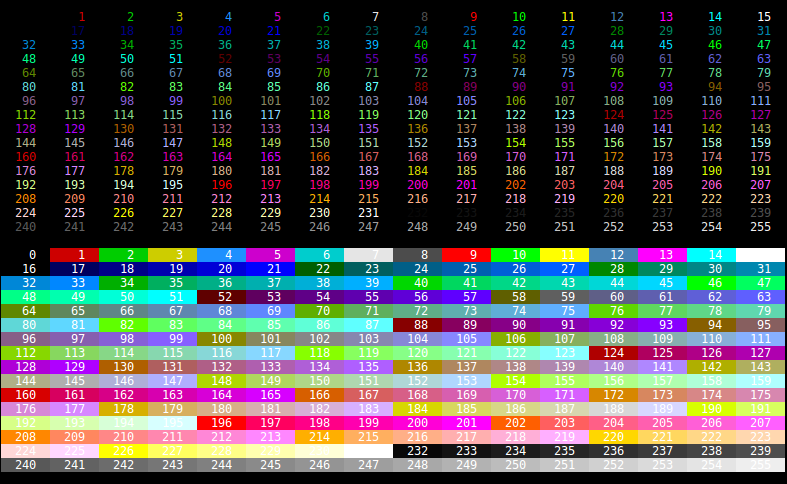
\includegraphics[width=0.95\textwidth, clip, trim=0 85mm 0 0]{ColoursTerminal}}
    \end{onlyenv}
    \begin{tikzpicture}[remember picture, overlay]
        \begin{scope}[scope on=<1>]
            \coordinate (yPos) at ($(8start)+(8mm,0mm)$);
            \foreach \n/\c in {8/PP, 16/PQ, 256/PS}{
                \draw[very thick, decorate, decoration={brace,amplitude=3pt}] (\n start -| yPos) ++(5mm,1mm) -- ($(\n end -| yPos)+(5mm,-1mm)$)
                      node[midway, right=2mm, text width=15mm, align=right, text=\c] {\n\ colours};
            }
            \node[anchor=north east, font=\ttfamily\large, rounded corners=1mm, draw=PP] at ($(current page.north east)-(8mm,4.5mm)$) {<Esc>[\tc{red}{FormatCode}m};
        \end{scope}
    \end{tikzpicture}
    \FrameRemark{$^\star$ GNOME Terminal 3.28 (VTE 0.52), debuting in Ubuntu 18.04 LTS, adds support for a \URL[PB]{https://askubuntu.com/a/985386}{few more styles}. Use code \PB{22} to unbold since \PB{21} is double underline!}
\end{frame}
%~~~~~~~~~~~~~~~~~~~~~~~~~~~~~~~~~~~~~~~~~~~~%
\begin{frame}[fragile]{Defining variables for colour codes}
    \vspace{-3mm}
    \begin{lstlisting}[style=MyBash, numbers=none]
        # Reset
        Default='\033[0m'
        # Regular Colors
        Black='\033[0;30m'
        Red='\033[0;31m'
        Green='\033[0;32m'
        Yellow='\033[0;33m'
        Blue='\033[0;34m'
        Magenta='\033[0;35m'
        Cyan='\033[0;36m'
        White='\033[0;37m'                 # Or you can wait to
        # Bold                             # learn about functions
        Bold='\033[1m'                     # and create your way!
        BBlack='\033[1;30m'
        BRed='\033[1;31m'
        BGreen='\033[1;32m'
        BYellow='\033[1;33m'
        BBlue='\033[1;34m'
        BMagenta='\033[1;35m'
        BCyan='\033[1;36m'
        BWhite='\033[1;37m'            # ...and so on and so forth!
    \end{lstlisting}
\end{frame}
%~~~~~~~~~~~~~~~~~~~~~~~~~~~~~~~~~~~~~~~~~~~~%
\begin{frame}[fragile]{Cursor movements}
    \vspace{-1mm}
    \begin{onlyenv}<1>
        In the same spirit of colours, the terminal cursor position can be moved:
        \smallskip
        \begin{description}[\texttt{<Esc><L>;<C>H}xxxxx]
            {\item[\texttt{<Esc>[<L>;<C>H}] Puts the cursor at line \texttt{L} and column \texttt{C}
            \item[\texttt{<Esc>[<L>;<C>f}] Puts the cursor at line \texttt{L} and column \texttt{C}
            \item[\texttt{<Esc>[<N>A}] Move the cursor up N lines
            \item[\texttt{<Esc>[<N>B}] Move the cursor down N lines
            \item[\texttt{<Esc>[<N>C}] Move the cursor forward N columns
            \item[\texttt{<Esc>[<N>D}] Move the cursor backward N columns
            \item[\texttt{<Esc>[2J}] Clear the screen, move to (0,0)
            \item[\texttt{<Esc>[K}] Erase to end of line
            \item[\texttt{<Esc>[s}] Save cursor position
            \item[\texttt{<Esc>[u}] Restore cursor position}
        \end{description}
    \end{onlyenv}
    \begin{onlyenv}<2>
        Use your imagination to take advantage of this functionality:
        \medskip
        \begin{lstlisting}[style=MyBash, numbers=none, xleftmargin=3mm, xrightmargin=3mm]
             $ while true; do
             >     printf "     $(date) \n\e[1A"
             >     sleep 1
             > done
             |+^C   Thu 11 Jul 18:07:26 CEST 2019+| # Stop it with CTRL-C
             
             # Here a crazy progress bar:
             $ while true; do
             >     printf '\e[s'
             >     printf '%0.s=' $(seq 1 $(bc -l <<< "$RANDOM/32767*100"))
             >     sleep 0.2
             >     printf '\e[u\e[K'  # Use \r instead of saving cursor
             > done
             |+======================^C+| # Stop it with CTRL-C
             
             $ printf 'You will never see my ${password}... MUAHAHA!\r\e[K'
             $
        \end{lstlisting}
    \end{onlyenv}
    \FrameRemark{The \bash|tput| command is a kind of wrapper for everything we learn in this section \,$\to$\,\URL[PB]{https://stackoverflow.com/a/20983251}{Starting point}}
\end{frame}

